\item \textbf{{[}HCI/PRELIM/9569/2021/P2/Q3{]}}

Name your Jupyter Notebook as 

\texttt{TASK3\_<your name>\_<centre number>\_<index number>.ipynb }

The task is to implement a priority queue using Object-Oriented Programming. 

A priority queue is an extension of queue with the following properties. 
\begin{itemize}
\item Every element has a priority associated with it. Smaller integer value
has a higher priority. 
\item An element with high priority leaves the queue before an element with
low priority.
\item If two elements have the same priority, they are served according
to their order in the queue, i.e. the earlier element will be served
before the later element (FIFO). 
\end{itemize}
For example, the emergency room in a hospital assigns patients with
priority numbers. The patient with the highest priority is treated
first, regardless of the order of arrival. 

An example of operations on a priority queue is shown below: 
\begin{center}
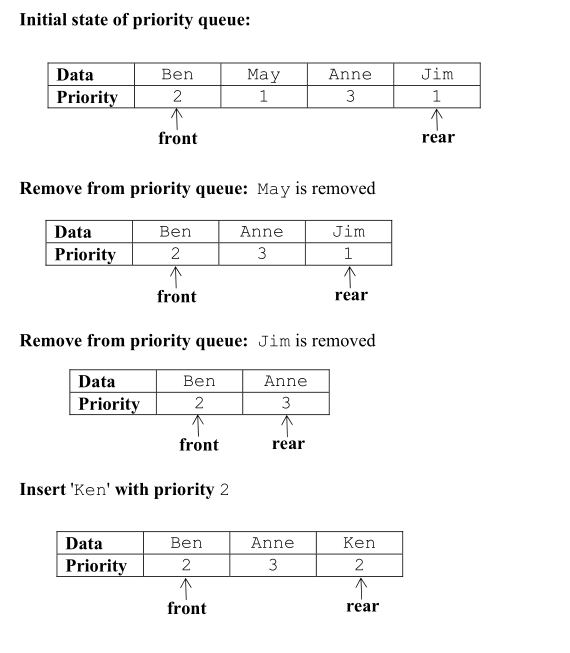
\includegraphics[width=0.5\paperwidth]{C:/Users/Admin/Desktop/Github/question_bank/LyX/static/img/9569-HCI-2021-P2-Q3-1}
\par\end{center}

A \textbf{priority queue} abstract data type (ADT) is to be implemented
as a linked list using object- oriented programming. Two classes \texttt{Node}
and \texttt{PQueue} have been identified.
\begin{center}
\begin{tabular}{|l|l|l|}
\hline 
\multicolumn{3}{|c|}{\texttt{Class: Node}}\tabularnewline
\hline 
\texttt{\hspace{0.01\columnwidth}}Identifier & \texttt{\hspace{0.01\columnwidth}}Data Type & \texttt{\hspace{0.05\columnwidth}}Description\tabularnewline
\hline 
\texttt{Data} & \texttt{STRING} & The node data\tabularnewline
\hline 
\texttt{Priority} & \texttt{INTEGER} & Indicates priority of node. Smaller value has higher priority\tabularnewline
\hline 
\texttt{Next} & \texttt{INTEGER} & Pointer to next node in queue.\tabularnewline
\hline 
\end{tabular}
\par\end{center}

\begin{center}
\begin{tabular}{|l|l|l|}
\hline 
\multicolumn{3}{|c|}{\texttt{Class: PQueue}}\tabularnewline
\hline 
\texttt{\hspace{0.01\columnwidth}}Identifier & \texttt{\hspace{0.01\columnwidth}}Data Type & \texttt{\hspace{0.05\columnwidth}}Description\tabularnewline
\hline 
\texttt{ThisPQueue} & \texttt{ARRAY{[}1:10{]} Of Node} & The priority queue data.\tabularnewline
\hline 
\texttt{Front} & \texttt{INTEGER} & Index for front node of queue.\tabularnewline
\hline 
\texttt{Rear} & \texttt{INTEGER} & Index for rear node of queue.\tabularnewline
\hline 
\texttt{NextFree} & \texttt{INTEGER} & Index for the next unused node.\tabularnewline
\hline 
\multirow{2}{*}{\texttt{Initialise()}} & \multirow{2}{*}{\texttt{PROCEDURE}} & - Set pointers to indicate all nodes are unused and linked. \tabularnewline
 &  & - Initialise values for \texttt{Front}, \texttt{Rear} and \texttt{NextFree}.\tabularnewline
\hline 
\multirow{2}{*}{\texttt{PQInsert(NewItem, Priority)}} & \multirow{2}{*}{\texttt{PROCEDURE}} & - Assign \texttt{NewItem} and \texttt{Priority} passed as parameters
to a node.\tabularnewline
 &  & - Insert the node to the rear of the priority queue.\tabularnewline
\hline 
\multirow{2}{*}{\texttt{PQDelete()}} & \multirow{2}{*}{\texttt{FUNCTION}} & - Remove a node of highest priority from the priority queue.\tabularnewline
 &  & - Return the \texttt{Data} attribute of the node that is removed.\tabularnewline
\hline 
\texttt{DisplayPQueue()} & \texttt{PROCEDURE} & Display the values of \texttt{Front}, \texttt{Rear}, \texttt{NextFree}
and the contents of \texttt{ThisPQueue} array in index order.\tabularnewline
\hline 
\end{tabular}
\par\end{center}

The diagram shows the linked list with: 
\begin{itemize}
\item the data items \texttt{'Ben'}, \texttt{'May'}, \texttt{'Anne'} and
\texttt{'Jim'} (inserted in that order) in the priority queue 
\item the unused nodes linked together 
\begin{center}
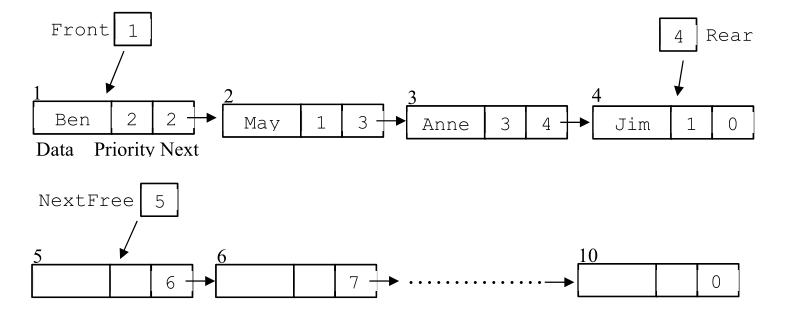
\includegraphics[width=0.5\paperwidth]{C:/Users/Admin/Desktop/Github/question_bank/LyX/static/img/9569-HCI-2021-P2-Q3-2}
\par\end{center}

\end{itemize}
For each of the sub-tasks, add a comment statement at the beginning
of the code using the hash symbol \textquoteleft \#\textquoteright ,
to indicate the sub-task the program code belongs to, for example: 
\noindent \begin{center}
\begin{tabular}{c|l|}
\cline{2-2} 
\multirow{2}{*}{\texttt{In{[}1{]}:}} & \texttt{\# Task 3.1}\tabularnewline
 & \texttt{Program Code}\tabularnewline
\cline{2-2} 
\multirow{2}{*}{\texttt{In{[}2{]}:}} & \texttt{\# Task 3.2}\tabularnewline
 & \texttt{Program Code}\tabularnewline
\cline{2-2} 
\multirow{2}{*}{\texttt{In{[}3{]}:}} & \texttt{\# Task 3.3}\tabularnewline
 & \texttt{Program Code}\tabularnewline
\cline{2-2} 
\multicolumn{1}{c}{} & \multicolumn{1}{l}{\texttt{Output:}}\tabularnewline
\end{tabular}
\par\end{center}

\subsubsection*{Task 3.1 }

Write program code for the classes \texttt{Node} and \texttt{PQueue},
including the \texttt{Initialise}, \texttt{PQInsert}, \texttt{PQDelete}
and \texttt{DisplayPQueue} methods. The code should follow the specification
given. \hfill{}{[}17{]}

\subsubsection*{Task 3.2 }

The program is to be tested. 

Write a main program to: 
\begin{itemize}
\item create a \texttt{PQueue} object 
\item read from file \texttt{PATIENTS.txt} all the data items with its priorities
into the priority queue by calling \texttt{PQInsert} method. 
\item output the priority queue by calling \texttt{DisplayPQueue} method.
\hfill{}{[}2{]}
\end{itemize}

\subsubsection*{Task 3.3 }

Write additional code in your main program to do the following in
order by calling the appropriate methods from \texttt{PQueue} class. 
\noindent \begin{center}
\begin{tabular}{|l|l|l|l|}
\hline 
No.  & Operation  & Data  & Priority\tabularnewline
\hline 
1  & Remove patient & \texttt{-} & \texttt{-}\tabularnewline
\hline 
2  & Remove patient  & \texttt{-} & \texttt{-}\tabularnewline
\hline 
3  & Add patient Carol & \texttt{Carol} & \texttt{4}\tabularnewline
\hline 
4  & Remove patient & \texttt{-} & \texttt{-}\tabularnewline
\hline 
5  & Remove patient & \texttt{-} & \texttt{-}\tabularnewline
\hline 
6  & Display priority queue  & \texttt{- } & \texttt{-}\tabularnewline
\hline 
\end{tabular}
\par\end{center}

Save your Jupiter Notebook for Task 3. \hfill{}{[}3{]}